\documentclass[a4paper,11pt]{article}
\input{/home/tof/Documents/Cozy/latex-include/preambule_lua.tex}
\newcommand{\showprof}{show them}  % comment this line if you don't want to see todo environment
\fancyhead[L]{Correction exercices graphes - parcours}
\newdate{madate}{10}{09}{2020}
%\fancyhead[R]{\displaydate{madate}} %\today
%\fancyhead[R]{Seconde - SNT}
%\fancyhead[R]{Première - NSI}
\fancyhead[R]{Terminale - NSI}
\fancyfoot[L]{~\\Christophe Viroulaud}
\AtEndDocument{\label{lastpage}}
\fancyfoot[C]{\textbf{Page \thepage/\pageref{lastpage}}}
\fancyfoot[R]{\includegraphics[width=2cm,align=t]{/home/tof/Documents/Cozy/latex-include/cc.png}}
\usepackage{tikz}
\usetikzlibrary{arrows}
\begin{document}
\begin{Form}
\begin{exo}
\begin{enumerate}
\item ordre: 8
\item $d_D=4$
\item Le graphe est connexe.
\item Parcours en profondeur (Les nœuds déjà dans la pile n'ont pas été ajoutés à nouveau):\\
\begin{center}
\begin{tabular}{|c|c|c|}
\hline 
nœud en cours & état de la pile & chemin parcouru \\ 
\hline 
D & G,A,B &  \\ 
\hline 
B & G,A,E & D \\ 
\hline 
E & G,A,F & D,B \\ 
\hline 
F & G,A,C & D,B,E \\ 
\hline 
C & G,A,H & D,B,E,F \\ 
\hline 
H & G,A & D,B,E,F,C \\ 
\hline 
A & G & D,B,E,F,C,H \\ 
\hline 
G &  & D,B,E,F,C,H,A \\ 
\hline 
 &  & D,B,E,F,C,H,A,G \\ 
\hline 
\end{tabular} 
\end{center}
\item Parcours en largeur du graphe (Les nœuds déjà dans la pile n'ont pas été ajoutés à nouveau):\\
\begin{center}
\begin{tabular}{|c|c|c|}
\hline 
nœud en cours & état de la file & chemin parcouru \\ 
\hline 
D & G,A,B &  \\ 
\hline 
B & E,G,A & D \\ 
\hline
A & C,E,G & D,B \\ 
\hline
G & C,E & D,B,A \\ 
\hline
E & F,C & D,B,A,G \\ 
\hline
C & H,F & D,B,A,G,E \\ 
\hline
F & H & D,B,A,G,E,C \\ 
\hline
H &  & D,B,A,G,E,C,F \\ 
\hline
 &  & D,B,A,G,E,C,F,H \\ 
\hline
\end{tabular} 
\end{center}
\end{enumerate}
\end{exo}
\begin{exo}
\begin{enumerate}
\item Cela revient à construire un graphe de 7 sommets dont chaque sommet correspond à une équipe. Comme chaque équipe doit en rencontrer 5 autres, alors chaque sommet serait de degré 5. Cependant la somme des degrés doit être pair (égale au double du nombre d'arêtes). Cette somme étant égale à 35, le tournoi n'est pas réalisable.
\item La somme des degrés est égale à 28. Le tournoi est réalisable. Il faut alors construire le graphe.
\begin{center}
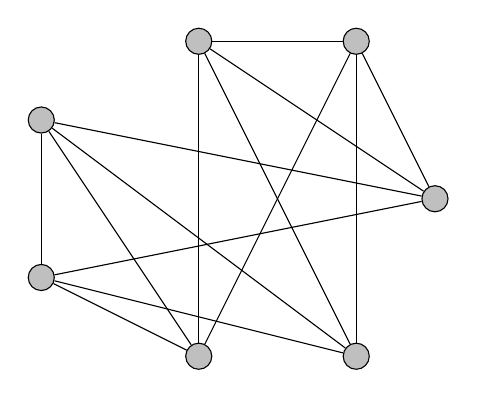
\begin{tikzpicture}
\node[draw,circle,fill=gray!50] (A)at(0,0) {};
\node[draw,circle,fill=gray!50] (B)at(2,0) {};
\node[draw,circle,fill=gray!50] (C)at(3,2) {};
\node[draw,circle,fill=gray!50] (D)at(2,4) {};
\node[draw,circle,fill=gray!50] (E)at(0,4) {};
\node[draw,circle,fill=gray!50] (F)at(-2,3) {};
\node[draw,circle,fill=gray!50] (G)at(-2,1) {};

\draw[-,>=latex] (A) -- (G);
\draw[-,>=latex] (A) -- (F);
\draw[-,>=latex] (A) -- (D);
\draw[-,>=latex] (A) -- (E);
\draw[-,>=latex] (B) -- (G);
\draw[-,>=latex] (B) -- (F);
\draw[-,>=latex] (B) -- (D);
\draw[-,>=latex] (B) -- (E);
\draw[-,>=latex] (C) -- (D);
\draw[-,>=latex] (C) -- (E);
\draw[-,>=latex] (C) -- (G);
\draw[-,>=latex] (C) -- (F);
\draw[-,>=latex] (D) -- (E);
\draw[-,>=latex] (F) -- (G);
\end{tikzpicture}
\captionof{figure}{Tournoi de handball}
\label{graphe}
\end{center}
\end{enumerate}
\end{exo}
\begin{exo}
\begin{center}
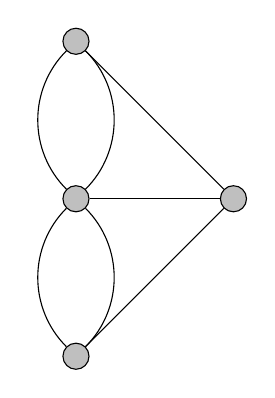
\begin{tikzpicture}
\node[draw,circle,fill=gray!50] (A)at(0,2) {};
\node[draw,circle,fill=gray!50] (B)at(0,0) {};
\node[draw,circle,fill=gray!50] (C)at(0,-2) {};
\node[draw,circle,fill=gray!50] (D)at(2,0) {};
\draw[-,>=latex] (A) to[bend left=-45] (B);
\draw[-,>=latex] (A) to[bend left=45] (B);
\draw[-,>=latex] (C) to[bend left=-45] (B);
\draw[-,>=latex] (C) to[bend left=45] (B);
\draw[-,>=latex] (B) -- (D);
\draw[-,>=latex] (A) -- (D);
\draw[-,>=latex] (C) -- (D);
\end{tikzpicture}
\captionof{figure}{Les sept ponts de Königsberg}
\label{graphe}
\end{center}
Tous les sommets sont de degrés impairs.
\end{exo}
\begin{exo}
\begin{enumerate}
\item DFS récursif
\lstinputlisting[firstline=12,lastline=17]{"scripts/dfs.py"}
\item Test
\item La méthode est tout aussi efficace: elle ne parcourt les arêtes qu'une seule fois.
\item Connexité
\lstinputlisting[firstline=19,lastline=21]{"scripts/dfs.py"}
\item DFS récursif avec un dictionnaire
\lstinputlisting[firstline=23,lastline=28]{"scripts/dfs.py"}
\item Chemin
\lstinputlisting[firstline=30,lastline=48]{"scripts/dfs.py"}
\end{enumerate}
\end{exo}
\begin{exo}
\begin{enumerate}
\item BFS avec un dictionnaire
\lstinputlisting[firstline=12,lastline=35]{"scripts/bfs.py"}
\item Cette fois il s'agit du plus court chemin.
\lstinputlisting[firstline=37,lastline=55]{"scripts/bfs.py"}
\end{enumerate}
\end{exo}
\end{Form}
\end{document}